\section{Initial Theory \& Background}
In terms of a Wireless Channel in the proposed Fall Detection System, it is preferred for the receiver to be able to estimate the state of the wireless channel. This can allow for optimisations to be made for optimal propagation of signals from transmitter to receiver. For the receiver to understand the state of the wireless channel, many models have been made which explain the properties and state of the channel.
\subsection{WLAN Channel Model}
%%%%%%%%%%%%%%%%%%%%%%%%%%%%%%%%%%%%%%%%%%%%%%%%%%%%%%%%%%%%%%%%%%%%%
A Wireless channel model describes how the amplitude and phase of a signal changes as it propagates from the transmitter to the receiver. Most important to me is the propagation model of a wireless channel and the two main propagation models are large-scale propagation known as large-scale path loss and small-scale propagation known as small-scale fading \citep{articleWLAN}. Doppler spread can also be considered. \par
To consider both of these, large-scale path loss describes the attenuation of the signal between the transmitter and receiver. In other words, it refers to the average loss in the signal's strength over a distance. Path loss for indoor environments of 5-10m between Tx \& Rx differ greatly from larger distances. It is caused by physical phenomena due to the environment such as reflection, diffraction, absorption and many more. As the physical environment constrains the wireless signals, the received signals conveys information that represents the environment that they pass through. It is clear that as the distance between transmitter and receiver is increased, the signal and thus, signal power, is spread over a larger area suffering greater attenuation. Small scale fading occurs due to the scattering environment between the transmitter and receiver caused by obstacles in the environment. It occurs when this scattering environment changes with time \citep{articleWLAN}. This leads to the transmitted signals scattering around the environment and arriving at the receiver whereby they are added constructively or destructively, as a function of time. This demonstrates the phase-shift in the wireless channel caused by the scattering environment. The signal level changes are called fading and has two types: microscopic \& macroscopic \citep{channelModels}\par
The scattering environment is composed of Line-of-Sight (LOS) and No-Line-of-Sight (NLOS) paths introduced by various factors such as furniture, walls, ceilings and more importantly in my case, people. Under a MIMO (Multi Input-Multi Output) system with multiple transmit and receive antennas, these effects due to the scattering environment are amplified. This is what is known as utilising the spatial diversity of the channel by sending symbols on different streams/links between one transmit antenna and one receive antenna. In reference to LOS and NLOS paths, a transmitted symbol through the LOS path will clearly arrive at the receiver before the corresponding symbol through a NLOS path (See Figure \ref{fig:LOS_NLOS}). Microscopic fading occurs when the receiver receives many copies of the signal due to scattering near the receiver while Macroscopic fading occurs receives multiple delayed copies of the signal due to the scattering environment over a large distance and time period (frequency selective fading). This is characterised by the delay spread of a channel which estimates earliest and latest arrival time of significant copies of the transmitted symbol \citep{channelModels, articleWLAN}  \par
As small-scale fading is a phenomenon when the scattering signal environment changes with time for smaller changes in the distance and multiple copies of the signal arriving at the receiver at once, it will be much more useful for this project. Transmitting distances are not long enough for large-scale path loss affect signal power greatly. \par
\begin{figure}[h]
\begin{center}
  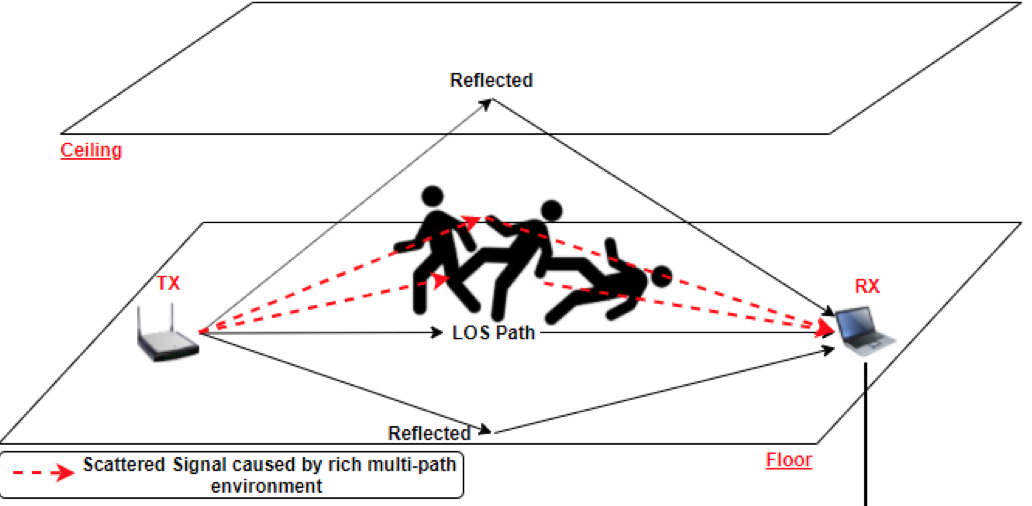
\includegraphics[scale=0.75]{Figures/Reflection.png}
\end{center}
  \caption{Demonstrates the LOS and NLOS paths between the Transmit and Receive antennas in a MIMO system. Note how the scattering environment is created due to the environment structure (floors, ceiling) and the person walking give rise to the phenomena of path loss and signal fading as discussed. Over a short LOS path, small-scale fading characterises the received signal and environment. (Diagram is taken from my Interim Presentation)}
  \vspace{-10pt}
  \label{fig:LOS_NLOS}
\end{figure}
A \textit{M} x \textit{N} (\textit{M} transmit and \textit{N} receive antennas) MIMO system can be modelled by the following equation at the receive antenna by a spatial vector \textbf{y} with a sampling period of T = 1/Bandwidth:
\vspace{-11pt}
\begin{equation}\label{eqn:2.1}
    \textbf{y}(k) = \textbf{H}(k)\textbf{x}(k)+\textbf{n}(k)
    \vspace{-11pt}
\end{equation}
where  $\textbf{x}(k) = \begin{bsmallmatrix}{x_1(k) & \cdots & x_M(k)}\end{bsmallmatrix}^T$ is the vector of transmitted signals, $\textbf{n}(k) = \begin{bsmallmatrix}{n_1(k) & \cdots & n_N(k)}\end{bsmallmatrix}^T$ is the AWGN (noise) vector for the channel and as mentioned before, $\textbf{H}(k)$ is the channel response matrix for the MIMO system at each time instance given by $k$.\citep{channelEquations}

\textbf{TALK abotu the baseband model and the model in euler form, then OFDM and the different modulation schemes and also how the bandwidth is influencing the various subcarriers. Talk abouthe 802.11n and OFDM}

  

%%%%%%%%%%%%%%%%%%%%%%%%%%%%%%%%%%%%%%%%%%%%%%%%%%%%%%%%%%%%%%%%%%%%%
%%%%%%%%%%%%%%%%%%%%%%%%%%%%%%%%%%%%%%%%%%%%%%%%%%%%%%%%%%%%%%%%%%%%%
\subsection{Channel State Information (CSI)}
\textbf{This is an estimation of the channel matrix H and is split into a different number of subcarriers depending on the bandwidth of the channel.From this we can obtain a characteristic of how the channel is behaving at a certain time. Speak about RSSI in the context of other papers and papers on indoor localisation and why it isnt correct to use it. Give the diagram from my presentation of the scattering signal} \\\\
%%%%%%%%%%%%%%%%%%%%%%%%%%%%%%%%%%%%%%%%%%%%%%%%%%%%%%%%%%%%%%%%%%%%%






%%%%%%%%%%%%%%%%%%%%%%%%%%%%%%%%%%%%%%%%%%%%%%%%%%%%%%%%%%%%%%%%%%%%%
%%%%%%%%%%%%%%%%%%%%%%%%%%%%%%%%%%%%%%%%%%%%%%%%%%%%%%%%%%%%%%%%%%%%%
\subsection{Obtaining CSI information}
\textbf{How do we obtain CSI information, csi information requires beamforming to be activated. we can use the Linux CSI tool developed with Intel and Microsoft and talk about how it returns data and link to the document that released it} \\\\
%%%%%%%%%%%%%%%%%%%%%%%%%%%%%%%%%%%%%%%%%%%%%%%%%%%%%%%%%%%%%%%%%%%%%




%%%%%%%%%%%%%%%%%%%%%%%%%%%%%%%%%%%%%%%%%%%%%%%%%%%%%%%%%%%%%%%%%%%%%
%%%%%%%%%%%%%%%%%%%%%%%%%%%%%%%%%%%%%%%%%%%%%%%%%%%%%%%%%%%%%%%%%%%%%
\section{Related Work \& Existing Fall Detection Systems}
\textbf{In this section, talk about the current work in the area and what they did to get any of it to work. However, then look at how each of them gathered the data classified after activity segmentation} \\\\
%%%%%%%%%%%%%%%%%%%%%%%%%%%%%%%%%%%%%%%%%%%%%%%%%%%%%%%%%%%%%%%%%%%%%






%%%%%%%%%%%%%%%%%%%%%%%%%%%%%%%%%%%%%%%%%%%%%%%%%%%%%%%%%%%%%%%%%%%%%
%%%%%%%%%%%%%%%%%%%%%%%%%%%%%%%%%%%%%%%%%%%%%%%%%%%%%%%%%%%%%%%%%%%%%
\subsection{Justification for Fall Detection Systems}
\textbf{talk here about the need for fall detection systems due to the amount of people falling each year/the amount of people who are causing the financial and health systems to be overloaded with falls} \\\\
%%%%%%%%%%%%%%%%%%%%%%%%%%%%%%%%%%%%%%%%%%%%%%%%%%%%%%%%%%%%%%%%%%%%%




%%%%%%%%%%%%%%%%%%%%%%%%%%%%%%%%%%%%%%%%%%%%%%%%%%%%%%%%%%%%%%%%%%%%%
%%%%%%%%%%%%%%%%%%%%%%%%%%%%%%%%%%%%%%%%%%%%%%%%%%%%%%%%%%%%%%%%%%%%%
\subsection{Wearable Approaches}
\textbf{Wearable approaches such as Accelerometers, phones, man down and what they have advantages and disadvantages. why they arent used. the privacy issues, the issue with people not wearing them} \\\\
%%%%%%%%%%%%%%%%%%%%%%%%%%%%%%%%%%%%%%%%%%%%%%%%%%%%%%%%%%%%%%%%%%%%%





%%%%%%%%%%%%%%%%%%%%%%%%%%%%%%%%%%%%%%%%%%%%%%%%%%%%%%%%%%%%%%%%%%%%%
%%%%%%%%%%%%%%%%%%%%%%%%%%%%%%%%%%%%%%%%%%%%%%%%%%%%%%%%%%%%%%%%%%%%%
\subsection{Ambient Environment Approaches} 
\textbf{The ambient environment issues in terms of infrared, floor vibration and sound sensors. sound is an iffy one because of how busy some of these environments are such as in a home. the TV could be on and there could be a false detection......floor vibration is expensive and useless tbh} \\\\
%%%%%%%%%%%%%%%%%%%%%%%%%%%%%%%%%%%%%%%%%%%%%%%%%%%%%%%%%%%%%%%%%%%%%




%%%%%%%%%%%%%%%%%%%%%%%%%%%%%%%%%%%%%%%%%%%%%%%%%%%%%%%%%%%%%%%%%%%%%
%%%%%%%%%%%%%%%%%%%%%%%%%%%%%%%%%%%%%%%%%%%%%%%%%%%%%%%%%%%%%%%%%%%%%
\subsection{Fall Detection using CSI}
\textbf{talk about any of the papers that have used it. first one will be WiFall, go through they use amplitude, how they get the data and how they organise it into different column arrays....talk about the frequency diversity and how it is actually impossible to limit it down, talk about the typical activity segmentation (what they use for activity detection), what they use for the classification and talk about how it is simply a binary decision \\ With Rt fall the decision is used to use the phase difference as it is a much more fine grainer use and this can be seen from Fila, E-eyes, perceiving accurate phase, what they used for each of it to get data or a model to train } \\\\
%%%%%%%%%%%%%%%%%%%%%%%%%%%%%%%%%%%%%%%%%%%%%%%%%%%%%%%%%%%%%%%%%%%%%





%%%%%%%%%%%%%%%%%%%%%%%%%%%%%%%%%%%%%%%%%%%%%%%%%%%%%%%%%%%%%%%%%%%%%
%%%%%%%%%%%%%%%%%%%%%%%%%%%%%%%%%%%%%%%%%%%%%%%%%%%%%%%%%%%%%%%%%%%%%
\subsection{Activity Segmentation}
\textbf{Now that I have considered each of the ways of doing it, how can i spot an activity of falling vs any of the others. Use RT Fall for this and WiFall....talka about the function that RTFall used and also how they can determine a fall vs any other. \\ In this section I need to note how the finishing points of each activity is needed and this goes into feature extraction which determines whether a fall, walking or anything is happening \\ Talk about other papers that use the CSI but not for fall detection and how they use it for their purpose \\ RELATE BACK TO FUTURE WORK SECTION} \\\\
%%%%%%%%%%%%%%%%%%%%%%%%%%%%%%%%%%%%%%%%%%%%%%%%%%%%%%%%%%%%%%%%%%%%%


%%%%%%%%%%%%%%%%%%%%%%%%%%%%%%%%%%%%%%%%%%%%%%%%%%%%%%%%%%%%%%%%%%%%%
%%%%%%%%%%%%%%%%%%%%%%%%%%%%%%%%%%%%%%%%%%%%%%%%%%%%%%%%%%%%%%%%%%%%%
\subsection{Classification of a Fall}
\textbf{Talk about the different classification techniques, how a 1 or 0 can be assigned in a binary classifier, as it is either a fall or no fall (walking or a fall like activity). Talk about their success rates and how others tried to improve on it. \\ RELATE BACK TO FUTURE WORK SECTION} \\\\















Citaat \cite{MScBuijs2010}

Citaat met pagina \cite[p.~10]{MScNugteren2010}

\url{http://en.wikibooks.org/wiki/LaTeX/}